\documentclass[a4paper,10pt,english]{book}

\usepackage[text={16cm,24cm},centering]{geometry}
\usepackage{calc}
\usepackage{ifthen}
\usepackage{epsfig}
\usepackage{palatino}
\usepackage{verbatim}
\usepackage{listings}
\usepackage{parskip}
\usepackage{array}
\usepackage{longtable}
\usepackage{amsmath}
\usepackage{hyperref}
\usepackage{parskip}
\usepackage{underscore}

\lstloadlanguages{C++,make,sh,csh}
\graphicspath{{images/}}
\hypersetup{colorlinks,raiselinks}

%------------------------------------------------------------------------
%   Simple commands
%------------------------------------------------------------------------


\renewcommand{\sectionautorefname}{Section}
\renewcommand{\subsectionautorefname}{Subsection}

\newcommand{\BlankLine}{\vspace{1.5ex} \noindent}
\newcommand{\Code}[1]{\texttt{#1}}
\newcommand{\Symbol}[1]{\textsl{#1}}
\newcommand{\Makexp}[1]{\texttt{\$(#1)}}


%------------------------------------------------------------------------
%   Listings commands and environments
%------------------------------------------------------------------------


\lstdefinestyle{default}
{
  basicstyle=\ttfamily, numbers=none, numberstyle=\tiny,%
  showstringspaces=false,
}

\lstdefinestyle{C++}
{
  style=default, language=C++
}

\lstdefinestyle{make}
{
  style=default, language=[gnu]make, showtabs=true
}

\lstdefinestyle{sh}
{
  style=default, language=sh
}

\lstdefinestyle{csh}
{
  style=default, language=csh
}

\lstnewenvironment{Source}[2][]
{
  \lstset{style=#2, xleftmargin=5mm, gobble=2, #1}
}
{}

\newcommand{\IncludeSource}[3][]
{
  \lstinputlisting[style=#2, frame=lines, firstline=2,%
                   aboveskip=\baselineskip,%
                   basicstyle=\small\ttfamily, #1]{#3}
}


%------------------------------------------------------------------------
%   Description environment
%------------------------------------------------------------------------


\newlength{\DescrLength}
\newcounter{DescrCounter}

\newcommand{\DescrFormat}[1]{#1}

\newcommand{\DescrLabel}[1]
{%
  \settowidth{\DescrLength}{\DescrFormat{#1}}%
  \ifthenelse{\lengthtest{\DescrLength > \labelwidth}}%
  {%
    \parbox[b]{\labelwidth}%
    {%
      \makebox[0pt][l]{\DescrFormat{#1}}\\\mbox{}%
    }%
  }{%
    {\DescrFormat{#1}}%
  }%
  \hfil\relax
  \refstepcounter{DescrCounter}
}


\newenvironment{Description}[1][\textnormal]
{
  \begin{list}{h}
  {
    \renewcommand{\DescrFormat}{#1}
    \renewcommand{\makelabel}{\DescrLabel}
    \setlength{\labelwidth}{30pt}
    \setlength{\itemindent}{0pt}
    \setlength{\leftmargin}{\labelwidth + \labelsep + \labelsep}
    \setlength{\rightmargin}{0pt}
  }
}
{ \end{list} }


%------------------------------------------------------------------------
%   MakevarTable environment
%------------------------------------------------------------------------


\newenvironment{MakevarTable}[1]
{
  \begin{longtable}[c]{|>{\ttfamily}lp{9.2cm}|}

    \caption*{#1}\\
    \hline
    \endhead

    \hline
    \endfoot

    JEM\_CXX\_OPT\_FLAGS1 & Rubbish \kill
}
{
  \end{longtable}
}



\begin{document}

\begin{titlepage}

  \begin{center}

    \vspace*{2cm}

    {\Huge \textsc{Jive user manual}}

    \vspace{1cm}

    {\large \textsc{version 2.0}}

    \vspace{2cm}

    {\large \textsc{Dynaflow Research Group}}

  \end{center}

\end{titlepage}

\tableofcontents


\chapter{Introduction}

Jive is an object oriented toolkit, written in C++, that can be used to
solve partial differential equations (PDEs). It provides a set of
functions and data structures -- bundled into \emph{classes} -- for
transforming a PDE into a system of equations; for solving such a system
of equations; and for computing quantities derived from the solution. In
particular, Jive provides classes for:
\begin{itemize}

\item storing and manipulating unstructured grids of arbitrary
  dimensions;

\item building dense and sparse matrices;

\item performing (sparse) matrix and vector operations;

\item solving linear systems of equations that may be subjected to sets
  of linear constraints;

\item solving non-linear and time-dependent PDEs;

\item evaluating the geometrical properties of basic shapes such as
  triangles, tetrahedra, hexahedra, and shapes of arbitrary
  dimensions;

\item reading/writing commonly used data structures from/to XML-formatted
  files;

\item running large-scale simulations on parallel computers;

\item and for visualizing 3-D data sets in real time.

\end{itemize}
Jive is not a ready-to-run program that computes an answer given a set of
input parameters. To make use of Jive you will have to write your own
program -- or modify an existing Jive program -- that computes the
solution of a particular PDE. This may take a more time than simply
starting a ready-to-run program, but it also enables you to tailor your
program to the PDE to be solved. What is more, Jive enables you to solve
virtually any type of PDE whereas ready-to-run programs are restricted to
a limited set of PDE types.

Although Jive has not been designed for one specific numerical method, it
currently provides most support for the finite element method. This does
not mean, however, that Jive can not be used in combination with other
numerical methods such as the finite difference method. In fact, most
components provided by Jive are useful for all common numerical methods.
Some of them can also be used to develop programs that do not solve a PDE
but perform other types of numerical operations, including data analysis
and data visualization.

%========================================================================

\section{User profile}

Jive is aimed at researchers who want or need to develop their own
programs for solving PDEs; for analyzing and processing data; for solving
large systems of (non-)linear equations; and for other types of numerical
computations. Jive is also aimed at students who want to gain practical
experience with various numerical methods for solving PDEs.

To use Jive you should have a working knowledge of the C++ programming
language. You should also have knowledge of common numerical methods such
as the finite difference method or the finite element method. Knowledge
of basic linear algebra algorithms, such as Gaussian elimination, is
recommended but not required.

%========================================================================

\section{Design overview}

Jive has been designed with five requirements in mind:
\begin{enumerate}

\item \textbf{portability}: Jive should be portable to all major
  operating systems and computer architectures.

\item \textbf{flexibility}: Jive should be flexible enough to implement
  state-of-the-art numerical solution procedures.

\item \textbf{ease of use}: Jive should be easy to use when developing a
  relatively simple application.

\item \textbf{modularity}: Jive should provide independent software
  components so that you only have to use those components that you
  really need.

\item \textbf{efficiency}: Jive should enable you to develop programs
  that make efficient use of the available computer resources.

\end{enumerate}
To meet the first requirement, Jive has been built on top of Jem, a C++
library that provides a portable interface to system-level services. Jem
also provides a collection of general-purpose functions and classes, such
as multi-dimensional arrays, that greatly simplify program development.
These functions and classes used to be part of Jive, but were later moved
to a separate library that is now named Jem. It is therefore no
coincidence that the structure of Jem is similar to the structure of
Jive.

To meet the second and third requirements, Jive provides both low-level
and high-level software components. The low-level components are generic
in nature and do not force you to structure your program in a particular
way. The high-level components, on the other hand, are more specific
in nature. They are more easy to use but they also force you to adopt a
specific design or solution procedure. By using the high-level components
you can quickly build a program that uses a ``standard'' procedure to
solve a PDE. By falling back to the low-level components you are also
able to implement a non-standard solution procedure or to customize part
of a standard solution procedure.

To meet the fourth requirement, Jive, like Jem, consists of largely
independent \emph{packages} containing collections of related classes and
functions. By using an event framework -- provided by the Jem library --
the classes within a package are also largely independent from each
other.

To meet the fifth and last requirement, Jive stores all large data sets
in large arrays. This means that the data can be accessed quickly and
that no additional memory is required for keeping track of the memory
addresses at which the data are stored.

%========================================================================

\section{Getting started}

Information about Jive is available from various sources: this user
manual, the online reference manual, the example programs that come with
Jive, and the web. The online reference manual consists of a set of HTML
pages that can be accessed from the main index page \Code{doc/index.html}
in the Jive installation directory and from the Jive website
(\JiveWebsite). The example programs can be found in the \Code{examples}
sub-directory in the Jive installation directory.

Since Jive uses components from the Jem library, you will have to be
somewhat familiar with the Jem library. Information about Jem can be
obtained from the Jem user manual; from the online reference manual; and
from the example programs that come with Jem. The online reference
manual can be viewed by opening the file \Code{doc/index.html} in the Jem
installation directory. The Jem reference manual is also accessible from
the Jive reference manual.

To start using Jive you are recommended to take the following steps:
\begin{enumerate}

\item Browse through the Jem user manual. You do not have to read it
  thoroughly from front to back; you only need to know how Jem is
  structured and what types of software components it provides.

\item Make yourself familiar with three concepts that are used frequently
  in Jive and that are implemented by Jem. These are: garbage collection;
  arrays and array expressions; and sparse matrices. In particular, you
  should read the documentation of the following classes: the
  \Code{Collectable} class; the \Code{Object} class; the \Code{Array}
  class; and the \Code{SparseMatrix} class. The documentation of these
  classes can be found in the online reference manual of Jem (the first
  three classes are part of the package \Code{base} and the last class is
  part of the package \Code{numeric}).

\item Read at least the next three chapters of this manual. The
  information provided by the other chapters is not strictly necessary to
  get started, but you may want to read these chapters to learn more
  about Jive.

\item Browse through the online reference manual to find out which
  classes are available. This will give you an impression of the
  capabilities of Jive.

\end{enumerate}

%========================================================================

\section{Outline of this manual}

\begin{comment}
  This manual is divided into three parts. The first part --
  Chapters~\ref{chapter:the-basics}
  to~\ref{chapter:extended-poisson-solver} -- explains how to start using
  Jive. After discussing some technical aspects of using Jive, it
  presents an elaborate example of a program that computes the solution
  of a simple PDE. The second part -- Chapters~\ref{chapter:utilities}
  to~\ref{chapter:io} -- focuses on the classes and functions
  provided by Jive. The aim of this part is to show which classes and
  functions should be used for which types of operations; to show how the
  classes are related to each other; and to explain why the classes have
  been designed the way they are. The third and last part --
  Chapters~?? to~?? -- discusses various numerical techniques that can be
  used to solve PDEs. It also shows how these techniques can be
  implemented efficiently with Jive.
\end{comment}

\textbf{\autoref{chapter:the-basics}} provides the technical
information that you need to know to write a program with Jive. In
particular, it explains what Jive is from a programmer's point of view;
how Jive is organized; how to use components from Jive -- and Jem --
in your program; how to use components from Jem in components from Jive
in your program; and how to compile and link your program.

\textbf{\autoref{chapter:essential-jem-components}} briefly describes the
essential classes from Jem that are used frequently in Jive. Basic
knowledge about these classes is required to start programming with Jive.

\textbf{\autoref{chapter:poisson-solver}} walks you through an
example program that uses the finite element method to compute the
solution of a simple Poisson problem. This chapter explains how you can
transform the PDE describing the Poisson problem into a linear system
of equations and how you can solve this system of equations.

\textbf{\autoref{chapter:mechanics-solver}} describes a more complex
example program that solves an elastic continuum mechanics problem
involving large deformations. This program illustrates how to solve a
non-linear PDE involving multiple unknowns with the finite element
method.

\begin{comment}

  \textbf{Chapter~\ref{chapter:utilities}} starts the second part of
  this manual by providing an overview of various general-purpose
  utility functions and classes. These include classes that represent
  unstructured grids/meshes; classes that represent the boundary of a
  grid/mesh; and classes that represent sets of nodes, elements,
  boundaries and other entities.

  Next, \textbf{Chapter~\ref{chapter:matrices}} focuses on matrices and
  vectors.  It indicates which classes in Jive -- and in Jem -- can be
  used to store vectors and various types of matrices; it shows which
  classes and functions can be used to perform common matrix/vector
  computations; and it explains how to extend Jive with new matrix
  classes and matrix/vector algorithms.

  After that, \textbf{Chapter~\ref{chapter:geom}} describes a family of
  classes that encapsulate the geometrical properties of basic shapes
  such as lines, triangles, and tetrahedra. You can use these classes to
  evaluate the shape functions of a finite element; to evaluate the
  gradients of the shape functions; to evaluate integrals over the
  domain of an element; and to evaluate other geometrical properties of
  a finite element, a finite volume cell, or some other geometrical
  entity.

  \textbf{Chapter~\ref{chapter:fem}} then deals with the classes and
  functions that have been designed specifically for finite element
  applications.  After reading this chapter, you will know which classes
  and functions can be used to implement a finite element model and to
  assemble a global matrix or vector.

  \textbf{Chapter~\ref{chapter:solvers}} provides an overview of the
  classes that can be used to solve (large) linear system of equations.
  It describes the strengths and weaknesses of these solver classes, and
  it indicates which solver should be used in a particular situation.
  This chapter also shows how one can apply a set of linear constraints
  to a system of equations.

  Finally, \textbf{Chapter~\ref{chapter:io}} describes the input/output
  framework provided by Jive and Jem. This framework consists of a
  collection of classes that can read and write commonly used data
  structures from and to XML-formatted files. Since these classes can be
  combined in an unlimited number of ways, you can easily define an
  input and output format that best matches the requirements of your
  application.

\end{comment}


\chapter{The basics; writing a program with Jive and Jem}
\label{chapter:the-basics}

This chapter focuses on the technical aspects of using Jive and Jem.
After reading this chapter you will know how to include components from
Jive and Jem into your source code and how to translate your source code
into an executable program.

Section~\ref{section:the-basics:using-components} starts this chapter by
explaining how to use the classes and functions provided by Jive and Jem.
It explains how Jive and Jem are organized; where to to find the header
file containing the declaration of a particular class or function; and
how to refer to the name of a class or function.
Section~\ref{section:the-basics:compilation} then shows how to compile
your program and how to link the resulting object file with the Jive and
Jem libraries. This section also shows how to simplify the compilation
and linkage procedure by using portable makefiles. Finally,
Section~\ref{section:the-basics:sample-program} presents a simple Jive
program together with a makefile.

%========================================================================

\section{Using classes and functions}
\label{section:the-basics:using-components}

From a programmer's point of view, Jive -- and Jem too -- consists of a
collection of C++ header files containing class and function declarations
and definitions. As usual, you include the contents of a header file by
putting an \Code{\#include} directive somewhere at the top of your source
file. To limit the header file sizes and to speed up the compilation of a
program, a header file typically contains only a single class definition
and/or a limited set of related functions. This implies that any
non-trivial program will have to include several header files, and that
you will have to know which header file contains which class/function
declaration.

%------------------------------------------------------------------------

\subsection*{Organization of Jive and Jem; working with packages}

Both Jive and Jem bundle related classes and functions into modular units
called \emph{packages}. For instance, the \Code{fem} package in Jive
contains all classes and functions that are aimed at developing finite
element programs. Except for a several core packages, most packages can
be installed and removed on an individual basis\footnote{This is not
entirely true because some packages depend on other packages.} so that
you can easily adapt Jive and Jem to your specific needs.

Here is an overview of the packages that are available in Jive:
\begin{Description}[\Code]

\item[util]    contains general utility classes, including classes for
  storing and manipulating unstructured grid.

\item[graph]   contains classes for partitioning graphs and for
  performing other operations on graphs.

\item[mp]      contains classes for exchanging data between parallel
  threads and processes.

\item[algebra] contains classes for storing and building sparse matrices,
  and for performing matrix/vector operations.

\item[geom]    contains classes for evaluating the geometrical properties
  of basic shapes and for computing element shape functions.

\item[model]   contains classes for implementing numerical models.

\item[app]     contains a modular, high-level application framework.

\item[gl]      contains classes for real-time data visualization.

\item[solver]  contains classes for solving linear systems of
  equations.

\item[fem]     contains classes that provide specific support for finite
  element applications.

\item[femodel] contains classes that implement finite element models.

\item[implict] contains classes for solving non-linear and time-dependent
  systems of equations.

\end{Description}

Jem provides the following packages that are used by Jive:
\begin{Description}[\Code]

\item[base]    contains foundation classes and functions.

\item[io]      contains classes for performing basic input and output
  operations.

\item[util]    contains general utility classes and containers such as
  hash tables.

\item[numeric] contains classes that provide support for numerical
  applications.

\item[mp]      contains classes for implementing parallel programs that
  are based on the message passing programming model.

\item[gl]      contains classes for managing and displaying scene
  graphs.

\item[xml]     contains classes for parsing and printing XML-formatted
  files.

\item[xutil]   contains special-purpose container classes.

\end{Description}

To use a class or function from a package you have to include the header
file containing the class or function declaration. By convention, all
header files provided by a Jive package are located in the directory
\Code{jive/}\Symbol{package-name} (assuming that the header file search
path of the compiler has been set up correctly; see the next section for
more information). Likewise, the header files provided by a Jem package
are located in the directory \Code{jem/}\Symbol{package-name}. The name
of the header file containing a particular class declaration can
generally be obtained by appending the suffix `\Code{.h}' to the name of
the class. Thus, the full pathname of the header file containing the
declaration of the class \Code{Constraints} in the package \Code{util} in
Jive is \Code{jive/util/Constraints.h}. Note that this rule is not
applicable to all classes; consult the reference manual to be sure.

%------------------------------------------------------------------------

\subsection*{Namespaces}

To avoid name collisions, all members (classes, functions, etc.) of a
Jive package are declared in the namespace
\Code{jive::}\Symbol{package-name}. The fully qualified name of the class
\Code{Constraints} in the Jive package \Code{util} is therefore
\Code{jive::util::Constraints}. Jem uses a similar naming scheme: all
members in a Jem package are declared in the namespace
\Code{jem::}\Symbol{package-name}. The members of the Jem package
\Code{base}, however, are declared in the namespace \Code{jem}. Thus, the
fully qualified name of the class \Code{String} from the \Code{base}
package is \Code{jem::String} and \emph{not}
\Code{jem::base::String}.

There are three ways to use names from a namespace: write the fully
qualified names; write one or more \emph{using declarations}; and write
one or more \emph{using directives}. The code fragment below shows an
example in which all three methods are used.

\IncludeSource{C++}{examples/namespaces.cpp}

Writing fully qualified names is the safest method because changes in one
part of your code can not lead to unexpected name collisions in another
part of your code. However, writing fully qualified names becomes tedious
pretty soon and also leads to code that is harder to read.

Using directives are at the other end of the spectrum: they minimize the
required typing effort, but they can also easily lead to name collisions
when you make small changes to your code. What is worse, changes in
external code, such as Jem, can also lead to name collisions in your own
code. Using directives should therefore only be used in small programs
with a limited lifespan.

Using declarations allow you to strike a balance between convenience
(less typing) and robustness (less chances for name collisions). They are
best used within functions, but for convenience you can also put them at
the top of your source files. You can also put them in header files, but
this increases the chances of name collisions. A better approach is to
create one header file -- named \Code{import.h}, for instance -- that
contains forward declarations and using declarations for names that you
use frequently throughout your program; see the example below.

\IncludeSource[title=\Code{import.h}]{C++}{examples/import.h}

Note that the header file \Code{import.h} uses forward class declarations
instead of including the header files containing the full class
definitions. This setup minimizes the compilation time for the source
files that include \Code{import.h} and use only some of those
classes.

%========================================================================

\section{Compiling and linking}
\label{section:the-basics:compilation}

Before you can run a Jive program -- or any C++ program -- you will have
to transform the source code into an executable program. This involves
two phases: compilation and linking. First, each source file is compiled
into a binary \emph{object file}. All the object files are then linked
with each other, with the Jive and Jem libraries, and with all other
required system libraries. The result of this linking process is an
executable program.

The next two sub-sections provide a more detailed description of the
compilation and linking processes when not using an integrated
development environment. The sub-section after that explains how you can
simplify the compilation and linking processes by using portable
makefiles. It is recommended that you read these three sub-sections, even
if you already are familiar with the compilation and linking
processes.

Some of the instructions given below involve the pathnames of the Jive
and Jem libraries. Since these libraries may be installed anywhere in a
filesystem, it is assumed that the environment variables \Code{JIVEDIR}
and \Code{JEMDIR} have been set to the full pathname of the Jive library
and Jem library, respectively. The notation \Code{\$JEMDIR} will be used
to refer to the value of the environment variable \Code{JEMDIR}.

%------------------------------------------------------------------------

\subsection*{The compilation procedure}

To compile a source file that includes components from Jive and/or Jem
you have to:
\begin{enumerate}

\item append the directory \Code{\$JIVEDIR/include} to the header file
  search path of the compiler;

\item append the directory \Code{\$JEMDIR/include} to the header file
  search path of the compiler;

\item append the necessary flags to the argument list of the compiler;

\item invoke the compiler.

\end{enumerate}
The command to compile a source file named \Code{source.cpp} typically
looks something like this:
\begin{verbatim}
  CC -I$JIVEDIR/include -I$JEMDIR/include -O -c source.cpp
\end{verbatim}
with \Code{CC} the name of the C++ compiler. The flag \Code{-O} indicates
that the compiler should turn on optimizations, and the flag \Code{-c}
indicates that the compiler should only produce an object file.

Although the above command will work with many compilers, some require
different and/or additional arguments. Consult the manual of your
compiler to make sure that you are using the correct arguments.

%------------------------------------------------------------------------

\subsection*{The linking procedure}

To create an executable program from one or more object files you have
to:
\begin{enumerate}

\item append the directories \Code{\$JIVEDIR/lib} and
  \Code{\$JEMDIR/lib} to the directory search path of the
  compiler;

\item append the directories of any non-standard libraries that are used
  to the directory search path of the compiler.

\item link your program with all your object files;

\item link your program with the required package-specific Jive
  libraries;

\item link your program with the required package-specific Jem
  libraries;

\item and link your program with the required system-specific libraries.

\end{enumerate}
Each package in Jem and Jive provides its own library containing all
object files related to that package. .When your program uses a class or
function from a package, you must link the program with the
package-specific library which is named \Code{jem}\Symbol{package} or
\Code{jive}\Symbol{package}. There are three exceptions: the packages
\Code{base}, \Code{io} and \Code{util} from Jem are combined in a single
library named \Code{jem}.

There are two ways to determine which system libraries are required. The
first one is to keep adding libraries until all symbols have been
resolved. Of course, you need to be fairly familiar with the system
libraries on your operating system for this scheme to work. Another,
and much more elegant way is to create a portable make file as is
explained in the next sub-section.

Note that the order in which the libraries are linked with the program is
significant with most linkers. In general, you should first list the Jive
libraries, then the Jem libraries, and then the system-specific
libraries.

%------------------------------------------------------------------------

\subsection*{Using portable makefiles}

To reduce the complexity of the compilation and linking process, each
package in Jive (and Jem too) provides a special makefile that specifies
which Jem/Jive libraries and which system libraries are required by that
package. They also specify which directories must be appended to the
header file search path and the library search path of the compiler. By
convention, a package-specific makefile is named
\Symbol{package-name}\Code{.mk} and is located in the directory
\Code{\$JIVEDIR/\-makefiles/\-packages} (or
\Code{\$JEMDIR/\-makefiles/\-packages}). The package-specific makefiles
rely on several features that are specific to GNU make. If GNU make
is not yet installed on your system, you can download a free copy from
the GNU website \url{www.gnu.org}.

You can use the package-specific makefiles by including them into your
own makefile. For instance, if your program uses the packages
\Code{solver} and \Code{fem} from Jive, you should put the following into
your makefile:
\begin{Source}{make}
  include $(JIVEDIR)/makefiles/packages/solver.mk
  include $(JIVEDIR)/makefiles/packages/fem.mk
\end{Source}

Note that the order of the include statements is not important. The
package-specific makefiles automatically resolve inter-package
dependencies, so you do not have to know that the package \Symbol{solver}
internally makes use of the package \Symbol{util}. This also works
between Jive and Jem packages. That is, a package-specific makefile from
Jive will automatically include the makefiles from the Jem packages on
which it depends. In the case that you are lazy and do not want to keep
track of which packages your program actually uses, you can simply put
this into your makefile:
\begin{Source}{make}
  include $(JIVEDIR)/makefiles/packages/*.mk
\end{Source}
But laziness has its price, and this construction may result in a
bunch of warnings from your compiler that some libraries are not used
to resolve any symbols.

When you include one or more package-specific makefiles into your
makefile, you still need some rules to actually build an executable (or
multiple executables) from your source files. Jive can help you out here,
provided that you only need to build a single executable. In this
case you only have to define the name of the executable, include all
required package-specific makefiles, and then include the makefile
\Code{\$JIVEDIR/\-makefiles/\-prog.mk}. The last makefile defines the
following rules:
\begin{Description}[\Code]

\item[\$(program)] builds an executable named \Makexp{program} by
  compiling and linking all C++ source files in the current directory.
  The variable \Code{program} must have been defined before the makefile
  \Code{\$JIVEDIR/\-makefiles/\-prog.mk} is included. This is the
  default make rule.

\item[opt] builds an optimized executable named
  \Makexp{program}\Code{-opt}. This executable will run faster than the
  standard one because it will perform less runtime checks.

\item[debug] builds an executable names \Makexp{program}\Code{-dbg} that
  contains debugging information.

\item[clean] deletes all object files and core dumps in the current
  directory. It also deletes any temporary files that may have been
  generated by the compiler.

\item[clean-all] invokes the \Code{clean} rule, and then deletes all
  executable programs.

\end{Description}

Your makefile may define a variable \Code{subdirs} that lists all
sub-directories containing source files that are part of your program.
You must define this variable before including the makefile
\Code{prog.mk} from Jive. Note that the names of your source files must
be unique; you can not have two source files with the same names that are
located in different sub-directories.

The package-specific makefiles define a (large) collection of variables
that can be used to write your own rules for compiling and linking
programs. The Jem reference manual provides a description of these
variables and explains how you can tune a makefile to your specific
needs.

%========================================================================

\section{A sample program}
\label{section:the-basics:sample-program}

The listing below contains the source code of a simple Jive program,
named \Code{linear}, that reads a data file, assembles and solves a
linear system of equations, and writes an output file. Do not worry if
you do not understand the details; the purpose of this program is not to
show what you can do with Jive but to show what a typical Jive program
looks like.

\IncludeSource[title=\Code{linear.cpp}]{C++}{examples/linear.cpp}

A makefile for this program is listed below. Note that only the makefile
from the \Code{implict} package needs to be included because this
makefile will include the makefiles from all other packages that are
needed.

\begin{Source}{make}
  program = linear
  include $(JIVEDIR)/makefiles/packages/implict.mk
  include $(JIVEDIR)/makefiles/prog.mk
\end{Source}


\chapter{Essential Jem components}
\label{chapter:essential-jem-components}

As Jive uses components from the Jem library, some knowledge of Jem is
required before you can start using Jive. This chapter therefore provides
a summary of the most frequently used classes and functions from Jem.
After reading this chapter you should be able to understand the example
programs presented in the next two chapters, and to make modifications to
these programs. Before you start implementing your own programs, however,
you are advised to consult the Jem user manual and reference manual. You
can skip this chapter if you are already familiar with Jem.

The classes and functions discussed in this chapter are divided into four
categories: core classes that form the foundation of Jem; utility classes
that implement various common data structures and algorithms; I/O classes
and functions that provide facilities for reading and writing data; and
numerical classes and functions that can be used to implement numerical
algorithms. Each category is dealt with in one of the following four
sections.

%========================================================================

\section{Core components}

The core classes and functions are located in the package \Code{base}.
They implement various basic data structures such as strings and arrays;
they provide support for memory management, multi-threading and
scripting; and they enable you to access various system-level services
in a portable way. The core classes that are used frequently in Jive are
summarized in \autoref{table:jem-core}. These classes are described in
more detail below.

\begin{table}

  \caption{Summary of the essential core classes.}
  \label{table:jem-core}

  \begin{center}

    \begin{tabular}{|>{\ttfamily}lp{10cm}|}
      \hline
      Name       & Description \\
      \hline \hline
      String      & Represents a character string. \\
      Slice       & Selects parts of array-like objects. \\
      System      & Provides access to the standard I/O streams
                    and other system facilities. \\
      Array       & Implements a multi-dimensional array that
                    supports slicing and array expressions. \\
      Collectable & Provides support for automatic garbage
                    collection. \\
      Ref         & Implements a `smart' pointer that points to a
                    collectable object. \\
      Object      & Defines a common base class for many
                    classes in Jem. \\
      Throwable   & Defines a base class for all exceptions thrown
                    by Jem and Jive. \\
      \hline
    \end{tabular}

  \end{center}

\end{table}


%------------------------------------------------------------------------

\subsection*{The \Code{String} class}

The \Code{String} class represents character arrays. It provides a set of
functions for accessing individual characters, for comparing strings, for
finding sub-strings, for transforming strings, and for creating string
slices (more about those in the next section). The \Code{String} class
also overloads the \Code{+} operator so that one can easily concatenate
two strings.

Strings are \emph{immutable}. This means that the individual characters
in a string can not be modified. The only way to change the contents of a
string is to call one of the assignment operators. You will have to use
an \Code{Array}, or a similar type of object, if you need to modify the
individual characters in a string. The \Code{StringBuffer} class can be
used to create strings with dynamic contents.

Note that the character array stored in a \Code{String} object is
\emph{not} null-terminated. Use the \Code{CString} class and the
\Code{makeCString} function to convert a \Code{String} object to a
null-terminated character array.

Below is a small example involving the \Code{String} class. Note that
some details, such as include directives and namespace declarations, have
been omitted to reduce the amount of code.

\IncludeSource{C++}{examples/String.cpp}

%------------------------------------------------------------------------

\subsection*{The \Code{Slice} class}

\Code{Slice} objects are used to select parts of arrays, strings, and
other array-like objects. Such a selection, or \emph{slice}, is defined
by three integers: a begin index, an end index and a stride. The begin
index is a non-negative integer that points to the first element in the
slice. The end index is an integer that points one position past the last
element in the slice. It is always larger than or equal to the begin
index. The stride is a positive integer that specifies the distance
between two consecutive elements in the slice. For instance, if the
stride is three, a slice contains only each third element of an
array-like object. If the stride equals one, the slice is said to be
contiguous.

Slices are created by invoking the so-called \emph{slice operator} of an
array-like object. This operator is a member function -- usually an
overloaded subscript or function call operator -- that accepts a
\Code{Slice} object and returns an object representing part of the
array-like object. The \Code{String} class, for instance, provides an
overloaded version of the subscript operator that returns a sub-string
for a given \Code{Slice} object.

\Code{Slice} objects are normally constructed by calling the non-member
function function \Code{slice()}, that is overloaded for several types of
slices (contiguous and non-contiguous slices, for instance). These
functions may be passed instances of the special classes
\Code{Begin}, \Code{End} and \Code{All} to create slices that start at
the beginning of an array, extend to the end of an array, or include all
elements of an array. For convenience, there are three pre-defined
instances of these classes which are named \Code{BEGIN}, \Code{END} and
\Code{ALL}, respectively. Note that the class \Code{All} is derived from
the \Code{Slice} class so an instance of this class can be passed
directly to a slice operator.

The following code fragment demonstrates how the \Code{Slice} class and
the \Code{slice()} function can be used to select slices from a
string.

\IncludeSource{C++}{examples/Slice.cpp}

%------------------------------------------------------------------------

\subsection*{The \Code{System} class}

The \Code{System} class provides access to various system-level
facilities. It can be used to get and set the standard input and output
streams; get information about the system; get the contents of
environment variables; and to catch and print exceptions thrown by
the main function of a program. Since it has only static members, it can
be viewed as a sort of mini namespace.

The \Code{System} class provides one input stream and four output
streams: one for writing error messages, one for writing warnings, one
for writing normal output, and one for writing log messages. The input
and output streams are initialized when they are accessed for the first
time.

The example code below prints a message to the standard output stream and
to the debug output stream (which is routed through the log output
stream). It then throws an exception that will be caught by the member
function \Code{System::exec}.

\IncludeSource{C++}{examples/System.cpp}

%------------------------------------------------------------------------

\subsection*{The \Code{Array} class}

The \Code{Array} class implements a multi-dimensional array of objects.
It is a class template with two template parameters. The first parameter,
say \Code{T}, specifies the type of the objects stored in the array. This
type should define at least a default constructor and a copy
constructor. The second parameter, say \Code{N}, specifies the
\emph{rank} -- i.e. the number of dimensions -- of the array. If the rank
parameter is omitted, a default value of one is assumed.

Each array has a \emph{shape}: an integer tuple (vector) of length equal
to the rank of the array. The elements of this tuple specify the sizes of
the array in each dimension. For instance, a three-dimensional array with
shape $(10,3,5)$ has size~10 in the first dimension, size~3 in the second
dimension and size~5 in the third dimension.

The elements in an array are identified in the usual way by a set of
integer indices ranging from zero to the corresponding array size minus
one. Thus, the index pair $(1,0)$ refers to the second element in the
first column of a two-dimensional array. The elements can be accessed by
means of the overloaded subscript and function-call operators.

An array stores its elements in a data block that may be shared with one
or more other arrays. As a consequence, multiple arrays may provide
different views to parts of the same data. For instance, a
one-dimensional array may provide access to a particular column of a
two-dimensional array. Another consequence of the shared storage scheme
is that the elements of one array may be modified through another
array.

The \Code{Array} class defines a set of slice operators -- overloaded
subscript and function-call operators -- that can be used to select
regular, rectangular sections of an array. These operators return an
\Code{Array} object that points to a sub-set of the data block pointed to
by the \Code{Array} object on which the slice operators are invoked.
Because the returned array shares its data with the original array, all
modifications to the returned array will be visible in the original
one, and the other way around.

Jem provides a set of overloaded operators and functions -- that are not
members of the \Code{Array} class -- for writing expressions that operate
on all elements of one or more arrays. These operators and functions
return special array objects, called \emph{array expressions}, that can
be assigned to regular \Code{Array} objects. Array expressions can also
be passed to the overloaded operators and functions to create new array
expressions. The use of array expressions is often more efficient than
writing a series of equivalent (nested) loops. One reason is that the
implementation of array expressions is based on `expression templates', a
technique that makes it possible to avoid creating temporary array
objects (see the papers available at \url{http://oonumerics.org} for the
details). Another reason is that array expressions collapse multiple
nested loops into a single loop in the common case that all the operands
are stored contiguously in memory.

The code fragment below demonstrates how to create an array, how to
access the elements of an array, how to create array slices and how to
make use of array expressions.

\IncludeSource{C++}{examples/Array.cpp}

%------------------------------------------------------------------------

\subsection*{The \Code{Collectable} and \Code{Ref} classes}

The \Code{Collectable} class provides support for automatic garbage
collection. That is, objects derived from the \Code{Collectable}, called
\emph{collectable objects}, are created on the heap and are automatically
deleted when they are no longer used. It is not possible to delete
collectable objects explicitly through a \Code{delete} expression.

Collectable objects are normally accessed through instances of the class
template \Code{Ref} that mimics the behavior of a pointer. As long as a
collectable object can be reached through a \Code{Ref} instance, or a
sequence of \Code{Ref} instances, that object will not be deleted.
Although one can also access collectable objects through normal pointers,
it is unspecified whether the existence of a route from a live pointer
(i.e. a pointer that can be reached from the program) to a
collectable object prevents the deletion of that object.

Collectable objects must be created with the function template
\Code{newInstance} that mimics a new expression but returns a \Code{Ref}
object instead of a normal pointer. The \Code{newInstance} function can
be supplied a variable number of arguments that will be passed on to the
matching constructor of the collectable class. A collectable object must
not be created on the stack. To prevent this from accidentally happening,
a collectable class should declare its destructor as a protected or
private member.

The example program below shows how to use the \Code{Collectable} and
\Code{Ref} classes. It defines and instantiates a trivial collectable
class, named \Code{Tracer}, that prints a message in its constructor and
destructor.

\IncludeSource{C++}{examples/Collectable.cpp}

This is the output of the program:

\begin{Verbatim}
  Tracer::Tracer  ( 1 )
  Tracer::Tracer  ( 2 )
  Tracer::~Tracer ( 1 )
  Tracer::~Tracer ( 2 )
\end{Verbatim}

When the \Code{Ref} object \Code{t2} is assigned to \Code{t1}, the first
\Code{Tracer} object is destroyed because no \Code{Ref} is pointing to it
any more; both \Code{t1} and \Code{t2} point to the second \Code{Tracer}
object. This object is destroyed when the function \Code{run} exits so
that both \Code{t1} and \Code{t2} are destroyed.

%------------------------------------------------------------------------

\subsection*{The \Code{Object} class}

Many classes in Jem are directly or indirectly derived from the class
\Code{Object}. It can therefore be used to implement heterogeneous
data structures and generic algorithms. For instance, a list
containing \Code{Object} instances can be used to store instances of
all classes derived from the \Code{Object} class. The \Code{Object}
class is derived from \Code{Collectable}, so that all \Code{Object}
instances are subjected to automatic garbage collection.

Jem provides two non-member functions that can be used to convert
non-\Code{Object} instances to \Code{Object} instances, and the other way
around. These two functions are named \Code{toObject()} and
\Code{toValue()}, respectively. This is illustrated in the following
example.

\IncludeSource{C++}{examples/Object.cpp}

%------------------------------------------------------------------------

\subsection*{The \Code{Throwable} class}

The \Code{Throwable} class defines a single base class for all exceptons
that are thrown by Jem and Jive. By convention, classes derived from the
\Code{Throwable} class provide a constructor with two string parameters:
one that describes the context in which the exception occured, and one
that describes the cause of the exception. These strings can be obtained
by calling the member functions \Code{where()} and \Code{what()},
respectively.

There are two families of exception classes: one derived from the
\Code{Exception} class and one derived from the \Code{RuntimeException}
class. The first family represents error conditions caused by external
events, such as wrong input, that a program should handle. The second
family represents error conditions caused by programming errors that
should not occur in an error-free program. Here is a brief example
demonstrating how to handle exceptions.

\IncludeSource{C++}{examples/Exception.cpp}

%========================================================================

\section{Utility components}

The package \Code{util} in Jem provides classes that implement various
types of containers such as lists, sets, and hash tables; that implement
an event framework with which you can connect independent software
components; that enable you to read, write and store configuration data
in a flexible way; and that provide various handy facilities.
\autoref{table:jem-util} lists the utility classes that are used
frequently in Jive. These classes are described in more detail in the
next few sub-sections.

\begin{table}

  \caption{Summary of the essential utility classes.}
  \label{table:jem-util}

  \begin{center}

    \begin{tabular}{|>{\ttfamily}lp{10cm}|}
      \hline
      Name        & Description \\
      \hline \hline
      ArrayBuffer & Implements an expandable array. \\
      SparseArray & Implements a multi-dimensional sparse array. \\
      Event       & Encapsulates a list of call-back functions
                    that are invoked when a specific event occurs. \\
      Properties  & Implements a hierarchical database containing
                    name/value pairs. \\
      \hline
    \end{tabular}

  \end{center}

\end{table}

%------------------------------------------------------------------------

\subsection*{The \Code{ArrayBuffer} class}

The class template \Code{ArrayBuffer} represents a one-dimensional array
that can grow and shrink. It is meant to be a helper class for creating
array objects of type \Code{Array<T,1>} of which the size is not known
beforehand. Here is an example:

\IncludeSource{C++}{examples/ArrayBuffer.cpp}

An \Code{ArrayBuffer} encapsulates a one-dimensional \Code{Array} object
that stores the elements in the \Code{ArrayBuffer}. The conversion of an
\Code{ArrayBuffer} to an \Code{Array} is therefore an efficient
operation.

%------------------------------------------------------------------------

\subsection*{The \Code{SparseArray} class}

The class template \Code{SparseArray} represents a multi-dimensional
sparse array. That is, an array that contains mostly zeroes, where the
definition of the term ``zero'' depends on the type of the array
elements. Although the interface of the \Code{SparseArray} class is
somewhat similar to that of the \Code{Array} class, it is intended to be
used as a storage container and not as a direct building block for
numerical algorithms. The \Code{SparseArray} class therefore does not
implement slice operators and does not provide support for sparse array
expressions.

Here is an example involving the \Code{SparseArray} class.

\IncludeSource{C++}{examples/SparseArray.cpp}

The output of the program will be like this:

\begin{Verbatim}
  1 0 0 0
  0 0 0 0
  0 0 0 2
  3 0 0 0
\end{Verbatim}

%------------------------------------------------------------------------

\subsection*{The \Code{Event} class}

The class template \Code{Event} encapsulates a list of call-back
functions, named \emph{delegates}, that are invoked when the
\Code{emit()} member function is called. Events can be used, among
others, to connect independent software components and to implement the
model-view-controller pattern. The template parameters of the
\Code{Event} class determine the parameter types of the \Code{emit()}
member function. These parameters are said to be the parameters of an
event. The number of parameters can be varied from zero to three, as
illustrated below:

\IncludeSource{C++}{examples/Event-1.cpp}

To be useful, an event should be connected to one or more delegates
by calling the non-member function \Code{connect()}. A delegate can be a
regular function or a non-static member function -- called a method
-- of a collectable class (that is, a class derived from the
\Code{Collectable} class). The parameter types of the delegate must be
compatible with the parameter types of the event. Thus, one can not
connect an event with a parameter of type \Code{int} to a delegate with
a parameter of type \Code{int*}. One can, however, connect an event to a
delegate that has less parameters than the event. In this case, the
last few parameters of the event will be discarded when the delegate
is called.

The example below illustrates the power of events. It involves two
independent classes that are connected to each other through an event.
The first class, named \Code{Graph} represents a graph that dynamically
displays a value as function of time. The second class, named
\Code{Sensor}, represents a device that measures some quantity at a given
location. Each time it has taken a new measurement, it calls the
\Code{emit()} member of its event named \Code{newValueEvent}. The
measurement is passed as an argument to the \Code{emit()} function that
passes it on to the member function \Code{addPoint()} of the \Code{Graph}
object that is connected to the event.

\IncludeSource{C++}{examples/Event-2.cpp}

%------------------------------------------------------------------------

\subsection*{The \Code{Properties} class}

The \Code{Properties} class implements an hierarchical database
containing a set of name/value pairs called \emph{properties}. It is
typically used as a repository for configuration data, but it can also be
used as a flexible in-memory data base.

The name of a property is represented by a \Code{String} instance. The
value of a property is a variable that has one of the following types:
\Code{bool}, \Code{int}, \Code{double}, \Code{String},
\Code{Array<bool>}, \Code{Array<int>}, \Code{Array<double>},
\Code{Array<String>}, or \Code{Object}. The value of a property can also
be a \Code{Properties} object so that you can build hierarchical sets of
properties. A \Code{Properties} object that is contained by another
\Code{Properties} object is called a \emph{nested} \Code{Properties}
object.

A \Code{Properties} object can be filled by calling the member functions
\Code{parseFile()} and \Code{parseFrom()}. The former reads a set of
properties from a file, while the latter reads a set of properties from
any text input stream. The contents of a \Code{Properties} object can be
printed by calling the member function \Code{printTo()} or by calling the
\Code{print} function.

Individual properties can be inserted into a \Code{Properties} object by
calling one of the overloaded versions of the \Code{set()} member
function. They can be extracted from a \Code{Properties} object by
calling one of the overloaded versions of the \Code{find()} or
\Code{get()} member functions. The difference between these two functions
is that the former does nothing if a property does not exist, while the
latter will throw an exception in that situation. Optionally, these
functions can check if the value of a property lies within a valid range.
The following code fragment illustrates how to set and get properties.
The last statement will throw an exception because the property named
``x'' does not exist.

A property can be inserted into or extracted from a nested
\Code{Properties} object by calling the \Code{set()}, \Code{find()} and
\Code{get()} functions with a \emph{compound property name}. Such a name
consists of a series of simple names concatenated by periods characters.
Here is an example:

\IncludeSource{C++}{examples/Properties-2.cpp}

The first statement inserts the integer property ``age'' into the nested
\Code{Properties} object named ``jones''. If this object does not exist
it is created on the fly. The second statement reads the double property
``length'' from the nested \Code{Properties} object named ``brown''. An
exception is thrown if this object does not exist.

%======================================================================

\section{I/O components}

The \Code{io} package exports classes for performing operations on
streams of text and binary data, and for getting information about files
and directories. \autoref{table:jem-io} lists the essential classes that
will be useful when developing applications with Jive.

\begin{table}

  \caption{Summary of the essential I/O classes.}
  \label{table:jem-io}

  \begin{center}

    \begin{tabular}{|>{\ttfamily}lp{10cm}|}
      \hline
      Name        & Description \\
      \hline \hline
      TextInput   & Defines an interface for reading text-based
                    input. \\
      TextOutput  & Defines an interface for writing text-based
                    output. \\
      Reader      & Represents a text input stream. \\
      Writer      & Represents a text output stream. \\
      PrintWriter & Formats a text output stream. \\
      \hline
    \end{tabular}

  \end{center}

\end{table}

%------------------------------------------------------------------------

\subsection*{The \Code{TextInput} class}

The \Code{TextInput} class defines an interface for reading data from a
text input stream. It is typically used to implement functions that parse
text input and that do not care about the source of the input. The
\Code{TextInput} class declares only abstract member functions; these
must be implemented by derived classes.

The non-member function \Code{read()} should be used to read objects from
a text input stream. Overloaded versions of this function are available
for reading fundamental objects such as integers and floating point
numbers, and for reading class instances, such as \Code{String} objects.
Multiple objects can be read in one statement by calling an overloaded
template version of the \Code{read()} function that has more than two
parameters. This is illustrated in the following example.

\IncludeSource{C++}{examples/TextInput.cpp}

%------------------------------------------------------------------------

\subsection*{The \Code{TextOutput} class}

The \Code{TextInput} class defines an interface for writing data to a
text output stream. It is essentially the opposite of the
\Code{TextInput} class.

The non-member function \Code{print()} should be used to write objects to
a text output stream. Overloaded versions of this function are available
for writing fundamental objects such as integers and floating point
numbers, and for writing class instances. Multiple objects can be written
in one statement by calling an overloaded template version of the
\Code{print()} function that has more than two parameters. This is
illustrated in the following example. Note that the special object
\Code{endl} is used to print a newline character.

\IncludeSource{C++}{examples/TextOutput.cpp}

%------------------------------------------------------------------------

\subsection*{The \Code{Reader} class}

The \Code{Reader} class implements the \Code{TextInput} interface and
provides various additional member functions for operating on text input
streams. Since the \Code{Reader} class is also derived from the
\Code{Object} class, \Code{Reader} objects are automatically destroyed
when they are no longer used.

The \Code{Reader} class does not specify where the input is coming from;
this is done by various derived classes, including:

\begin{Description}

  \item[StringReader] reads data from a \Code{String} object.

  \item[FileReader] reads data from a text file.

  \item[GzipFileReader] reads data from a compressed text file.

\end{Description}

%------------------------------------------------------------------------

\subsection*{The \Code{Writer} class}

The \Code{Writer} class implements the \Code{TextOutput} interface and
provides various additional member functions for operating on text output
streams. It is the opposite of the \Code{Reader} class. In fact, many
classes derived from the \Code{Reader} class have a corresponding
class that is derived from the \Code{Writer} class.

The example below shows how to convert a text file into a compressed text
file using the \Code{FileReader} and \Code{GzipFileWriter} classes. Note
that an exception will be thrown if the input file does not exist.

\IncludeSource{C++}{examples/Writer.cpp}

%------------------------------------------------------------------------

\subsection*{The \Code{PrintWriter} class}

The class \Code{PrintWriter} can be used for writing formatted text
output. It provides control over the maximum width of each line, the
indentation level and the way that numbers are formatted. It is to be
used as a wrapper around a \Code{Writer} object the specifies where the
formatted output should go, as illustrated in the following example. Note
that the public member object named \Code{nformat} contains the settings
for formatting numbers.

\IncludeSource{C++}{examples/PrintWriter.cpp}

The output of the above code will look like this:

\begin{Verbatim}
  Thank you for visiting ShopUntilYouDrop! We hope that you will
  enjoy your new goodies and that we will see you again soon.

  Here is a summary of your purchase:

    Number of items  ......      4
    Price per item   ......  42.24
    Total amount     ......  169.0

  Bye bye!
\end{Verbatim}

%======================================================================

\section{Numerical components}

The \Code{numeric} package contains classes and functions for building
numerical algorithms. They can be used to multiply matrices and vectors;
to solve linear systems of equations; to define and evaluate functions;
and to perform various other types of operations. The essential functions
and classes are listed in \autoref{table:jem-numeric}.

\begin{table}

  \caption{Summary of the essential numerical classes and functions.}
  \label{table:jem-numeric}

  \begin{center}

    \begin{tabular}{|>{\ttfamily}lp{10cm}|}
      \hline
      Name         & Description \\
      \hline \hline
      matmul       & \\
      MatmulChain  & \\
      LUSolver     & \\
      SparseMatrix & \\
      Function     & \\
      \hline
    \end{tabular}

  \end{center}

\end{table}



%
\chapter{Implementation of a Poisson solver}
\label{chapter:poisson}

The aim of this chapter is to introduce the classes that make up the
foundation of Jive. To this end, it walks you through an example
program that uses the finite element method to compute the solution of
a Poisson problem. The example program demonstrates how to build a
finite element mesh; how to convert the PDE describing the Poisson
problem into a linear system of equations; and how to solve that
system of equations.

\BlankLine
This chapter starts with a brief description of the Poisson problem
and its boundary conditions.
Section~\ref{section:poisson:solution-procedure} then describes
how the Poisson problem can be solved by means of the finite element
method. This section also introduces some of the terminology that is
used in the remaining sections.  After that,
Section~\ref{section:poisson:class-summary} provides a summary
of the classes from Jive and Jem that are used in the example program.
The aim of this section is to reduce the amount of new information
that is presented in the following sections.
Section~\ref{section:poisson:program-structure} then summarizes
the structure of the example program. Next,
Sections~\ref{section:poisson:mesh-construction}
to~\ref{section:poisson:solution} describe how the example
program builds a mesh, assembles the linear system of equations, and
solves that system of equations.
Section~\ref{section:poisson:complete-program} ends this
chapter by listing the main function of the example program.

\BlankLine
The Poisson problem is defined on a two-dimensional, rectangular
domain~$\Omega$ with boundary $\Gamma = \DirichletBoundary \cup
\NeumannBoundary$, as illustrated in Figure~\ref{fig:poisson-problem}.
Homogeneous Dirichlet boundary conditions are prescribed
on~\DirichletBoundary, while homogeneous Neumann boundary conditions
are prescribed on~\NeumannBoundary. The mathematical formulation of
the problem is given by the following three equations:
\begin{displaymath}
  \begin{alignedat}{2}
    - \nabla^{2} u(\bm{x}) & = f(\bm{x}) \, , \qquad
      & \bm{x} & \in \Omega. \\
    u(\bm{x}) & = 0 \, , \qquad
      & \bm{x} & \in \DirichletBoundary. \\
    \bm{n} \Inproduct \bm{\nabla} u(\bm{x}) & =  0 \, , \qquad
      & \bm{x} & \in \NeumannBoundary.
  \end{alignedat}
\end{displaymath}
where the scalar $u$ is the state variable, $\bm{x}$ is the spatial
coordinate, $\Nabla$ is the gradient operator, and $f$ is a given
function. The vector~$\bm{n}$ is the normal on the Neumann
boundary~\NeumannBoundary.
\begin{Figure}

  \begin{center}
    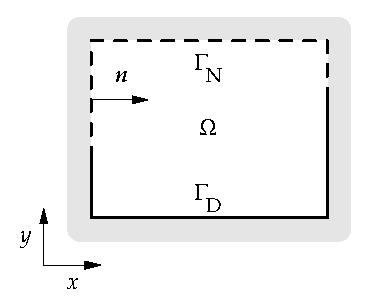
\epsfig{file=figures/poisson-problem.eps}
  \end{center}

  \caption{A schematic representation of the Poisson problem. The
    symbol~$\Omega$ denotes the spatial domain,
    \DirichletBoundary~denotes the Dirichlet boundary,
    \NeumannBoundary~denotes the Neumann boundary, and $\bm{n}$
    denotes the normal vector on~\NeumannBoundary.}

  \label{fig:poisson-problem}

\end{Figure}


%======================================================================

\section{The solution procedure}
\label{section:poisson:solution-procedure}

To solve the Poisson problem by means of the finite element method,
the PDE is first replaced by its equivalent weak formulation: find the
state $u$ such that
\begin{displaymath}
  \Int{\Omega} v \nabla^{2} u \, \Dee\Omega +
  \Int{\Omega} v f \, \Dee\Omega = 0
\end{displaymath}
for all continuous test functions $v$ which are zero
on~\DirichletBoundary. Using the divergence theorem, the weak
formulation can also be written as: find $u$ such that
\begin{displaymath}
  - \Int{\Omega} \Nabla v \Inproduct \Nabla u \, \Dee\Omega +
  \Int{\Omega} v f \, \Dee\Omega = 0
  \label{eq:poisson-weak}
\end{displaymath}
For all continuous test functions $v$.


%----------------------------------------------------------------------

\Signpost{Approximation by polynomial functions}

The next step in the finite element method is to approximate the state
$u$ by a set of polynomial functions. This is done by creating a
\emph{mesh} comprising a set of \emph{elements} and \emph{nodes}. The
elements -- numbered from one to~$n_e$ -- are obtained by dividing the
spatial domain~$\Omega$ into sub-domains $\Omega_{e_i}, i \in \{1,
\ldots, n_e\}$, as is illustrated in Figure~\ref{fig:poisson-mesh}.
The nodes -- numbered from one to~$n_n$ -- are obtained by defining a
set of points on the edges of the elements. Or, stated differently,
each element is assigned a set of nodes which it shares with other
elements.
\begin{Figure}

  \begin{center}
    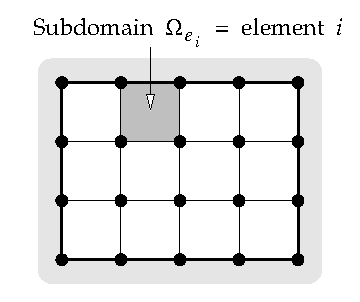
\epsfig{file=figures/poisson-mesh.eps}
  \end{center}

  \caption{A sample mesh for the Poisson problem.}

  \label{fig:poisson-mesh}

\end{Figure}

\BlankLine
In each element~$i$, the solution of the Poisson problem is
approximated by a polynomial function~$\hat{u}$ that is given by:
\begin{displaymath}
  \hat{u}(\bm{x}) = \bm{N}_{e_i}(\bm{x}) \, \bm{a}_{e_i} \, , \ \bm{x}
  \in \Omega_{e_i}.
\end{displaymath}
The matrix $\bm{N}_{e_i}$ contains the interpolation polynomials, or
\emph{shape functions}, of element~$i$.  Its dimensions are $1 \times
|e_i|$, where $|e_i|$ denotes the number of degrees of freedom
attached to element~$i$ (which, in this particular case, equals the
number of nodes attached to element~$i$).  The vector $\bm{a}_{e_i}$
contains the (unknown) values of the state in the nodes of the
element.

If the values of the state in all nodes of the mesh are collected in
one large vector~$\bm{a}$, then the above equation can also be written
as:
\begin{displaymath}
  \hat{u}(\bm{x}) = \bm{N}_{e_i}(\bm{x}) \, \bm{L}_{e_i} \bm{a}
  \, , \qquad \bm{x} \in \Omega_{e_i}.
\end{displaymath}
The matrix $\bm{L}_{e_i}$ is a sparse, boolean matrix with dimensions
are $|e_i| \times n_n$. It is called the \emph{location operator} of
element~$i$ because it extracts an element vector from a global
vector. That is, it extracts a vector defined on the nodes of an
element from a vector defined on all nodes of the mesh.

An approximation of $\Nabla u$ can be obtained by applying the
gradient operator to the previous equation. This yields:
\begin{equation}
  \Nabla \hat{u}(\bm{x}) = \bm{G}_{e_i}(\bm{x}) \, \bm{L}_{e_i} \bm{a}
  \, , \qquad \bm{x} \in \Omega_{e_i}
  \label{eq:poisson-gradient-approximation}
\end{equation}
where the matrix $\bm{G}_{e_i}$ contains the spatial derivatives of the
element shape functions. It has $|e_i|$ columns and as many rows as
the number of spatial dimensions (two in this case).

The test functions~$v$, which are used in the weak formulation, are
constructed in the same way as the approximate solution~$\hat{u}$.
This means that within each element~$i$
\begin{displaymath}
  v(\bm{x}) = \bm{N}_{e_i}(\bm{x}) \, \bm{L}_{e_i} \bm{w} \, ,
  \qquad \bm{x} \in \Omega_{e_i}
\end{displaymath}
where the global vector~$\bm{w}$ contains the values of the test
functions within the nodes of the mesh. The gradient of the test
functions are obtained simply by replacing the matrix $\bm{N}_{e_i}$
by the matrix $\bm{G}_{e_i}$.


%----------------------------------------------------------------------

\Signpost{Transformation into a system of equations}

The Poisson problem is now transformed into a linear system of
equations by substituting the polynomial approximations
into the weak formulation~(\ref{eq:poisson-weak}) of the Poisson
problem. This yields:
\begin{eqnarray*}
  - \Int{\Omega} \Nabla v \Inproduct \Nabla u \Dee\Omega +
  \Int{\Omega} v f \, \Dee\Omega
  & \approx & \\
  \sum_{i = 1}^{n_e} \left(
    - \Int{\Omega_{e_i}} \Nabla v \Inproduct \Nabla \hat{u} \,
    \Dee\Omega +
    \Int{\Omega_{e_i}} v f \, \Dee\Omega
  \right) & = & \\
  \sum_{i = 1}^{n_e} \left(
    - \Int{\Omega_{e_i}} (\bm{G}_{e_i} \bm{L}_{e_i} \bm{w})^{T}
    \bm{G}_{e_i} \bm{L}_{e_i} \bm{a} \, \Dee\Omega +
    \Int{\Omega_{e_i}} \bm{N}_{e_i} \bm{L}_{e_i} \bm{w} f \, \Dee\Omega
  \right) & = & \\
  \bm{w}^T \sum_{i = 1}^{n_e} \left(
    - \Int{\Omega_{e_i}} \bm{L}_{e_i}^{T} \bm{G}_{e_i}^{T}
    \bm{G}_{e_i} \bm{L}_{e_i} \, \Dee\Omega \, \bm{a} +
    \Int{\Omega_{e_i}} \bm{L}_{e_i}^{T} \bm{N}_{e_i}^{T} f \,
    \Dee\Omega
  \right) & = & 0
\end{eqnarray*}
Since the above equality must hold for all possible vectors~$\bm{w}$,
the final expression between the brackets must be equal to zero.
This means that the vector~$\bm{a}$ is the solution of
\begin{displaymath}
  \left(
    \sum_{i = 1}^{n_e} \Int{\Omega_{e_i}}
    \bm{L}_{e_i}^{T} \bm{G}_{e_i}^{T} \bm{G}_{e_i} \bm{L}_{e_i} \,
    \Dee\Omega
  \right) \bm{a} =
  \sum_{i = 1}^{n_e} \bm{L}_{e_i}^{T} \left(
    \Int{\Omega_{e_i}} \bm{N}_{e_i}^{T} \, f \, \Dee\Omega
  \right)
\end{displaymath}
which can be written as
\begin{equation}
  \bm{K} \bm{a} = \bm{f}.
  \label{eq:poisson-linear-system}
\end{equation}
The matrix $\bm{K}$ is a $(n_n \times n_n)$ sparse matrix that is
called the \emph{global matrix}. It is assembled element-wise as
follows:
\begin{displaymath}
  \bm{K} = \sum_{i = 1}^{n_e} \bm{L}_{e_i}^{T} \left(
    \Int{\Omega_{e_i}} \bm{G}_{e_i}^{T} \bm{G}_{e_i} \, \Dee\Omega
  \right) \bm{L}_{e_i} =
  \sum_{i = 1}^{n_e} \bm{L}_{e_i}^{T} \bm{K}_{e_i}
  \bm{L}_{e_i}.
\end{displaymath}
The matrix~$\bm{K}_{e_i}$ is a $(|e_i|\times |e_i|)$ dense matrix that
is called the \emph{element matrix} of the $i$-th element. The
vector~$\bm{f}$ has length $n_n$ and is called the \emph{global
  right-hand side} vector. Like the global matrix it is constructed
element-wise:
\begin{equation}
  \bm{f} = \sum_{i = 1}^{n_e} \bm{L}_{e_i}^{T} \left(
    \Int{\Omega_{e_i}} \bm{N}_{e_i}^{T} \, f \, \Dee\Omega
  \right)
  = \sum_{i = 1}^{n_e} \bm{L}_{e_i}^{T} \, \bm{f}_{e_i}.
  \label{eq:global-righ-hand-size}
\end{equation}
The vector $\bm{f}_{e_i}$ is called the \emph{element right-hand side}
vector of the $i$-th element. Its length is equal to $|e_i|$.

\BlankLine
Since the solution of the Poisson problem must satisfy the Dirichlet
boundary conditions, all components of $\bm{a}$ corresponding with the
nodes on the Dirichlet boundary must be equal to zero. If these
prescribed components are numbered last, then the system of
equations~(\ref{eq:poisson-linear-system}) can be written as:
\begin{displaymath}
  \left[
    \begin{array}{cc}
      \bm{K}_{11} & \bm{K}_{12} \\
      \bm{K}_{21} & \bm{K}_{22}
    \end{array}
  \right] \left[
    \begin{array}{c}
      \bm{a}_{1} \\
      \bm{0}
    \end{array}
  \right] = \left[
    \begin{array}{c}
      \bm{f}_{1} \\
      \bm{f}_{2}
    \end{array}
  \right]
\end{displaymath}
in which the vector $\bm{a}_{1}$ contains all unknown, non-prescribed
components of $\bm{a}$. The unknown components are therefore obtained
by calculating the solution of
\begin{displaymath}
  \bm{K}_{11} \, \bm{a}_{1} = \bm{f}_{1}.
\end{displaymath}


%======================================================================

\section{Outline of the program}
\label{section:poisson:program-outline}


%======================================================================

\section{Construction of the mesh}
\label{section:poisson:mesh-construction}


%======================================================================

\section{Assembly of the global system of equations}
\label{section:poisson:assembly}


%======================================================================

\section{Solution of the global system of equations}
\label{section:poisson:solution}


%======================================================================

\section{The complete program}
\label{section:poisson:complete-program}


\end{document}
